% LLNCS macro package for Springer Computer Science proceedings;
% Version 2.20 of 2017/10/04
\documentclass[runningheads]{llncs}

\usepackage{graphicx}
\graphicspath{{images/}}
\usepackage{todonotes}
\usepackage{float}

% Necessary to be able to use urls in the bib file
\usepackage{url}

% Used for displaying a sample figure. If possible, figure files should
% be included in EPS format.
%
% If you use the hyperref package, please uncomment the following line
% to display URLs in blue roman font according to Springer's eBook style:
% \renewcommand\UrlFont{\color{blue}\rmfamily}

%
% Extra commands for references
%
\newcommand{\appendixref}[1]{Appendix~\ref{#1}}
\newcommand{\figureref}[1]{Figure~\ref{#1}}
\newcommand{\sectionref}[1]{Section~\ref{#1}}
\newcommand{\subsectionref}[1]{Subsection~\ref{#1}}
\newcommand{\chapterref}[1]{Chapter~\ref{#1}}
\newcommand{\tableref}[1]{Table~\ref{#1}}
\newcommand{\formularef}[1]{Formula~\ref{#1}}

\begin{document}

\title{An approach for continuous painting detection and room prediction during a museum walk}
%
%\titlerunning{Abbreviated paper title}
% If the paper title is too long for the running head, you can set
% an abbreviated paper title here
%
\author{
    Thomas Aelbrecht \and
    Andreas De Witte \and
    Jochen Laroy \and
    Pieter-Jan Philips \and
    Gillis Werrebrouck
}

% The short form of the title
\titlerunning{Continuous painting detection in a museum}

% The short form of the authors
\authorrunning{T. Aelbrecht et al.}
% First names are abbreviated in the running head.
% If there are more than two authors, 'et al.' is used.
%
\institute{Ghent University, Valentin Vaerwyckweg 1, 9000 Ghent, Belgium}
%
\maketitle              % typeset the header of the contribution
%
\begin{abstract}

Are you tired of exploring a museum on a map and figuring out where you are? This paper focusses on resolving this issue. It allows the detection of paintings in a video or on a live recording while walking through the museum. The paintings are detected using a mean-shift segmentation filter, floodfilling and contour detection. The detected paintings are matched against all known paintings in the museum and a couple of predictions are made. These predictions are then used as input for a model inspired by the Hidden Markov model which determines if the given predictions are possible and don't cause a teleportation through the museum. All information is displayed on a clear map so it's easy to know where you are in the museum. Never look at the map again, look at your phone while enjoying the paintings!

\keywords{Painting detection \and Painting matching \and Painting mask \and Hidden Markov model}
\end{abstract}
%

% TODO: content here
\section*{Introduction}

This paper focusses on describing the different steps to reconstruct the path of an excursion through a museum. The first section describes how the paintings are cut out of high-quality pictures. The following section explains an algorithm that can independently find paintings in a picture. Prior research has been done on this topic, one of which is by He et al. \cite{he2019scan}. This paper focusses on the detection of irregularly shaped objects in images and was used as inspiration for the automatic mask creation in the detection algorithm further described in this document. The third section is about how paintings are being matched which was inspired by the work of Liu et al. \cite{liu2020image}. This section describes performant solutions to figure out which paintings are visible in a picture. The fourth section is about how to localize where a person is. This is done by using a custom implementation of the Hidden Markov model to decide which location is a logical result. This model was designed by consolidating the concepts of a paper about a basic Hidden Markov model \cite{eddy1996hidden}, one about speech recognition \cite{juang1991hidden} and a paper about combining historic probabilities \cite{genest1986combining}. The fifth and final section is about the visualization of the result. This section describes a modern way of visualizing the visited rooms in the museum.

\section{Semi-supervised painting detection}
\label{sec:assignment1}

\subsection{The naive painting detection algorithm}
\label{subsec:contour_detection}
The contour detection is the actual logic part of the semi-supervised painting detection. This is the part that decides what contours are in the image and it works as described below.

Before any contour detection can be done, as many unnecessary details as possible have to be removed. OpenCV has several options to solve this problem, for example erode, dilate, blurring (median, Gaussian\dots) or downscaling. The image needs to get rid of as many details as possible to prevent detection of contours inside the paintings or on the wall. Although this won't be perfect, the removal of details will decrease the number of incorrectly detected contours.

So the first step of the algorithm is to remove details by resizing the image. Our implementation scales the image down and back up with a factor 5. To scale the image back up, pixel values are calculated using the pixel area. The scale up was mostly done to be able to show the original image, but it's also a possibility to use the algorithm with the downscaled image. This will result in a slight increase in performance because the image it's working on would be smaller.

The next step is to convert the image to grayscale. This is done to make it easier to differentiate certain parts. This grayscaled image is then dilated and eroded to remove even more noise at the borders of the painting or on the walls. The last step of removing noise is to do a median blur over it. The biggest advantage of using median blur is that it will preserve edges while removing noise. The idea behind these steps is to smeare as many details as possible, in other words to make bigger blots with the same color. This makes it easier to detect the borders and remove noise in the background.

The next step is to detect edges with Canny. The result of the Canny function will then be dilated once again to make the found edges stronger. After this the contours can be detected using OpenCV's algorithm. This algorithm will make sure only the most outer contours are returned when a hierarchical structure of contours is found. A small final detail to prevent unlogical solutions is the following: any contour with a ratio smaller than 1:10 will be removed. This prevents very small contours to appear around noisy parts of the image.

\subsection{Strengths and weaknesses}

This biggest strength of this algorithm is that it will give an output in almost every image. An example of an image where no painting will be detected is an image where the framework of the painting is not visible, meaning the image only contains the painting itself, no wall and no framework. With this kind of paintings, the desired sulution is a contour containing the entire painting, while this is not possible because the painting has no border at all. Another advantage is that the algorithm is very fast in detecting contours due to the fact that all the parts of the algorithm are standard functions that have a good performance.

However, the biggest weakness of this algorithm is that almost every found contour is not precise enough, so almost every solution needs a slight adjustment. For some solutions, the algorithm detects contours that are slightly larger than the actual painting, while for other paintings, it doesn't even include the border of the painting.

Another weakness of the algorithm is that paintings sometimes have overexposure or shadows, which makes it harder to detect it's contours. Some paintings even have a small tag with a description next to the painting, sometimes this small tag is detected as being a painting. This is a logical decision, because there's a big contrast in colors and the tag has a clear contour, but this is not a desired effect.

This algorithm is a first version to quickly be able to fill the database with the groundtruth. The actual algorithm in its final version is completely different and doesn't have these issues anymore.

% \chapter{Assignment 2}
\section{Unsupervised painting detection}
\label{sec:unsupervised_painting_detection}
The algorithm in assignment 2 drastically differs from the algorithm in assignment 1 (see \sectionref{sec:contour_detection}), it was designed from scratch with the weaknesses of the previous algorithm in mind.

The first step in the algorithm is a mean shift segmentation (see \ref{fig:paiting_detection_mean_shift})). This is a method to remove noise by taking the mean of the pixels within a certain range. A big advantage is that it partialy removes color gradients and fine-grain textures which would cause issues in the further steps of the algorithm.

\begin{figure}[h]
    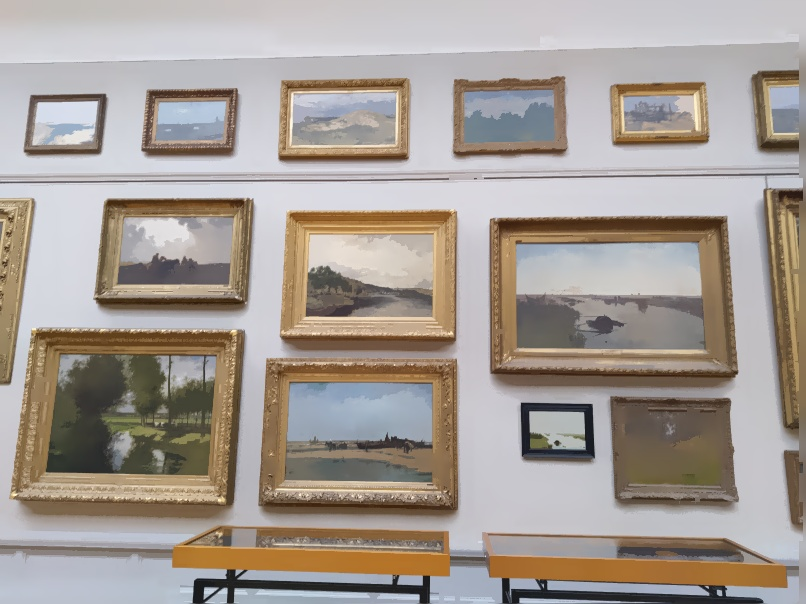
\includegraphics[width=\linewidth]{images/IMG_20190323_121447_mean-shift.jpg}
    \caption{Mean shift segmentation.}
    \label{fig:paiting_detection_mean_shift}
\end{figure}

A common technique in object detection is by creating a mask of the object. The problem with this is that we aren't certain about the size and ratio of the paiting as well as where the painting is located in the image and how many there are in the image. This can be solved by thinking the other way around. The one certainty that is consistent throughout all images is that all paintings hang on a wall. A mask for the wall will be made instead of making a mask for the paintings. The mask of the painting(s) can then be obtained by simply inverting the mask.

Another issue is that this mask can't be statically programmed in code for each image since we wan't to be able to use the algorithm on any image or video frame. This can be solved by using a technique called flooding. Flooding will create a mask from a starting position in the image and will fill all neighbouring pixels if they have a color close to the color of the starting position. This is done recursively until no pixels are withing the color range of the starting position anymore.

\begin{figure}[h]
    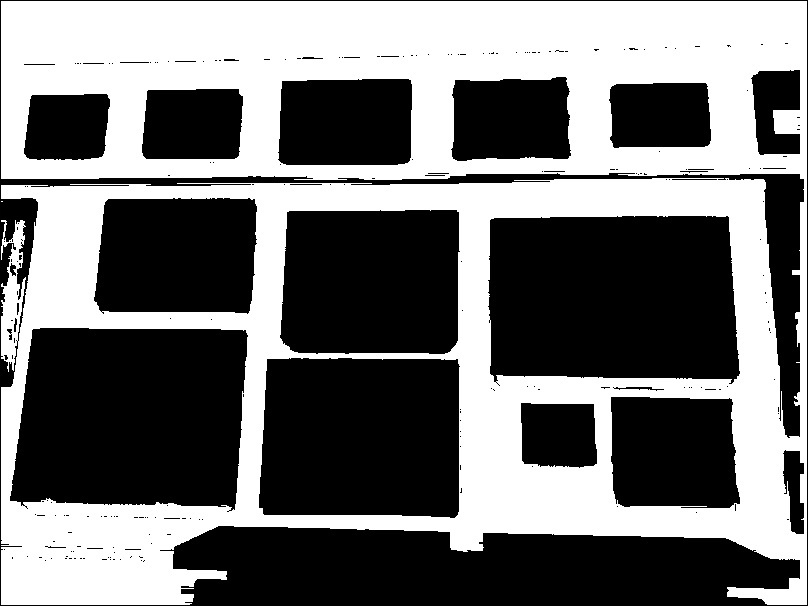
\includegraphics[width=\linewidth]{images/IMG_20190323_121447_wall-mask.jpg}
    \caption{Wall mask.}
    \label{fig:paiting_detection_wall-mask}
\end{figure}

The next problem is that there needs to be a good starting position to have a good and correct mask for the wall. To find this, the unsupervised algorithm will iterate over all pixels of the image with a certain step size and perform floodfill with that pixel as starting position. Once a mask is found that has the same height and width as the image, then this is the mask that will be used. If no such mask is found after iterating over all pixels (with a certain step size), then the mask with the bigest size is used. This is because sometimes part of the floor or other elements in the image will obstruct the floodfill algorithm to find a mask that has the same size of the image. See \ref{fig:paiting_detection_wall-mask}) for an example of such mask.

Once the mask of the wall has been obtained, it is inverted to have the mask of the paintings (see \ref{fig:paiting_detection_paintings-mask}). The mask is then eroded to remove small imperfections in the mask and a median blur is used to smooth the edges of the mask.

\begin{figure}[h]
    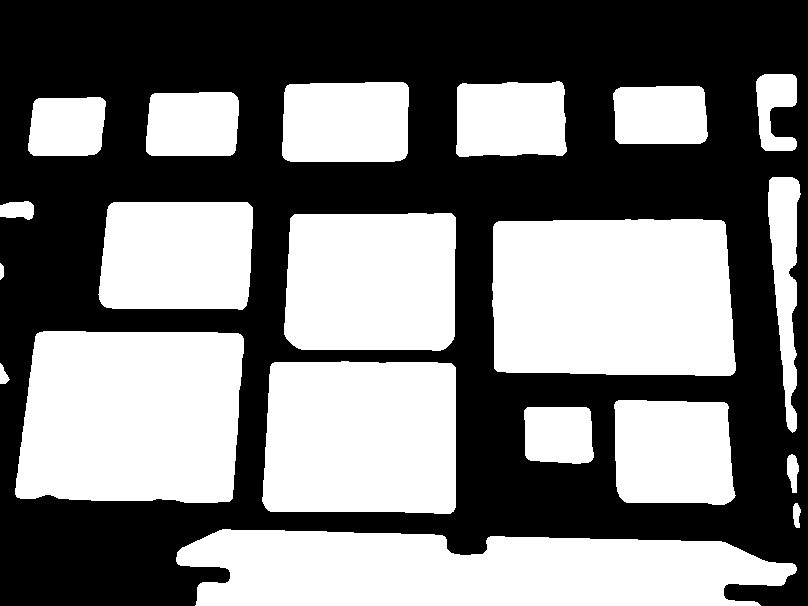
\includegraphics[width=\linewidth]{images/IMG_20190323_121447_paintings-mask.jpg}
    \caption{Paintings mask.}
    \label{fig:paiting_detection_paintings-mask}
\end{figure}

The next step is to use Canny, the difference with the naive approach is that the two threshold values are determined by using the Otsu algorithm to choose the optimal threshold value.

Next, a morphological transformations is performed on the Canny edges (see \ref{fig:paiting_detection_paintings-edges}). This will close edges that are close to each other as this will improve the detection of closed contours. This morphological transformations is in essence a dilation followed by an erosion.

\begin{figure}[h]
    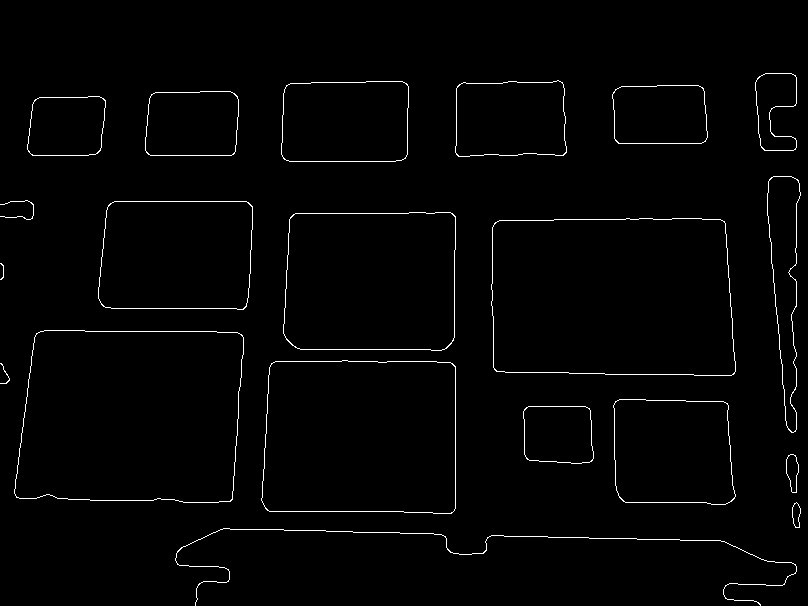
\includegraphics[width=\linewidth]{images/IMG_20190323_121447_edges.jpg}
    \caption{Paintings edges.}
    \label{fig:paiting_detection_paintings-edges}
\end{figure}

The next steps are exactly the same as the naive painting detection algorithm as described before. The contours are detected in the Canny edges and only fully enclosed polygons with 4 sides are returned as quadrilaterals.

\subsection{Strengths and weaknesses}

The most important improvement of the detection algorithm is that it isn't based on smearing out colors and finding contours in it anymore. The key to success with this algorithm is the use of automatic mask creation by using floodfill as main technique. Most of the paintings are detected in most of the images. The detected paintings also have a better fit compared to the naive algorithm.

Most paintings in the dataset are correctly detected as well those in the test set. Only on some occasions there is a miss detection. One flaw that has been found is that some doorways are detected as a painting. This is logical because of how the mask creation works with the floodfilling. In the case of such a detection flaw, the doorways obstructs the floodfilling algorithm to correctly create a mask of the non-painting area. This is something that doesn't happen too often.

A minor problem that the algorithm has, which is also the case in the naive algorithm, is that it sometimes detects dark shadows as part of the painting. Although, this is less of an issue in this algorithm then it was in the naive algorithm. It doesn't affect the accuracy too much because if there is a shadow, it only appears on one side of the painting and it doesn't reach far.

A drawback of this algorithm is that it is less performant than the naive algorithm. This is mainly because of the mask creation, specifivally the floodfilling. There has been a slight performace gain by using threading for this but it still remains slower. A possiblity to resolve this and speed up the algorithm would be to use GPU processing power to perform the mask creation. NVidia for example has Cuda cores on which algorithms can be preformed many times faster than on CPUs. This is not possible for this project because OpenCV (developed by Intel) in Python doesn't have the possiblity to execute on GPU's.

\section{Quantitative comparison}
In order to make a quantitative comparison, two things are needed. First of all, the quadrilaterals have to be found autonomously (as described in \sectionref{sec:contour_detection}). The second thing needed is the groundtruth of the dataset which has been generated by using the solution created in assignment 1 (see \chapterref{chap:assignment1}).

To measure the accuracy of the painting detection algorithm, 3 things are required; the amount of false negatives (= paintings that are not found at all), the amount of false positives (= detected paintings that aren't paintings) and the bounding box accuracy (= average intersection divided by union).

With the creation of the solution for this problem, a new problem occurs: how to find the intersection of these two shapes? The solution to this problem is made by using ``Shapely''. To do so, the quadrilaterals have to be transformed into a polygon. Once this is done, ``Shapely'' can compute the intersection. It has been tested whether this gives correct intersections if two polygons are not intersecting, or when they are sharing only a line. Also some more general intersections have been tested. Once the intersection is made, it's easy to find the area of the polygon, using ``Shapely'' once again.

For each of the presumably perfect paintings, all of the found quadrilaterals are checked. The intersection is made and when the ``intersection divided by union'' is bigger than the previous maximum, than a new best match is found. In the end, when all found quadrilaterals have been tested, a check is done whether the area of the intersection is existing. If this is the case, this value is added to the average intersection divided by union parameter and the amount of found paintings is incremented. If this was not the case, than a painting that needs to be found was not found and the amount of false negatives is incremented. After all of the paintings from the database are checked, the average intersection divided by union parameter is divided by the amount of paintings found. Also, the amount of false positives is calculated by subtracting the amount of paintings found from the amount of quadrilaterals.

The accuracy results for the detection algorithm were fairly good. An example of the detection can be seen in \ref{fig:paiting_detection_with_ground_truth}. Red is the detected contours and blue is the groundtruth as determined with the use of assignment 1. The dataset consists of 553 images which all together contain 836 paintings. The detection algorithm had 68 false negatives (paintings) and 35 false positives (paintings). The average bounding box accuracy is 82.80\%.

\begin{figure}[h]
    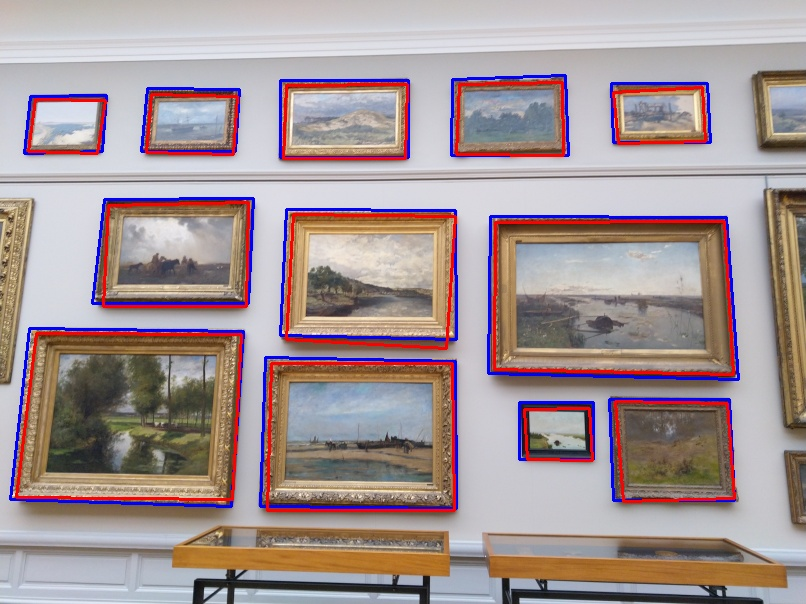
\includegraphics[width=\linewidth]{images/IMG_20190323_121447.jpg}
    \caption{Paintings detection.}
    \label{fig:paiting_detection_with_ground_truth}
\end{figure}

\section{Qualitative evaluation}

\section{Matching}
\label{sec:matching}

\subsection{Features}
\label{subsec:the-features}

Before diving deeper into the matching algorithm, it's important to explain the features that are used to do the matching. The algorithm only depends on two types histograms of the detected paintings. The first type is a histogram of the full painting, the second type is a collection of histograms gathered from different blocks of the painting. The block sized used in this algorithm divides the painting in 4 rows by 4 columns (or 16 blocks), independent of the painting's size. Both features are saved to the database for each of the labeled paintings and are both used in the matching algorithm explained in the next section.

\subsection{The matching algorithm}
\label{subsec:matching-algo}

The first step in matching a given painting with the entire dataset of paintings is a light intensity equalization. This way different light intensities have no influence on the histograms gathered from a detected painting. Equalization is a technique that is only used on the video frames because of the rather bad frame quality, the dataset itself and the previously performed benchmarks don't need this step. \cite{patel2013comparative}

The second step consists of fetching the histograms as described in \sectionref{subsec:the-features}. Thereafter these histograms are compared against all histograms in the dataset. Per known painting the distance between the histograms is calculated using a technique called \emph{correlation}. This way a chance between 0 and 1 is obtained. The histogram of the whole painting gives one chance, the block histogram gives a total of 16 chances which are combined by taking the average. These two chances are combined using \formularef{eq:histogram-score} which calculates a weighted average. In this formula, $P(X = P_{i})$ stands for the chance that the detected painting $X$ is painting $P_{i}$ from the dataset, $B$ stands for the average of the block histogram distances and $F$ stands for the distance of the normal histograms. The block histogram gets a much higher weight because the predictions with these histograms are much more reliable than these with the normal histograms.

\begin{equation}
    \label{eq:histogram-score}
    P(X = P_{i}) = \frac{(8 * B) + (1 * F)}{9}
\end{equation}

The matching algorithm gives a list of possible rooms with the according chances per detected painting, even if the room is not accessible given the current room. How impossible rooms are treated, will be explained in \sectionref{sec:localization}. The algorithm has also an option to ignore chances that are below a given threshold.

\subsection{Matching results}
The matching algorithm has been tested in three ways. First, the dataset was matched against itself without using the detection algorithm but by using the corners from the semi-supervised algorithm. The result for this test is that 835 of 836 paintings were matched correctly. This means that only one painting could not be uniquely matched, this could be because some paintings appear in multiple images. The average matching probability is 92.24\%.

The second test was performed on the dataset but in combination with the detection algorithm described in \sectionref{subsec:detection-algo}. The result for this is that 702 of the 762 detected paintings were matched correctly.

The third and last test was performed on the test dataset also in combination with the detection algorithnm. The images have been divided in folders with the correct room as name to be able to count the amount of correct room matches. The result for this test is that 158 of the 338 detect paintings had a correct room match. This is lower than the dataset because these images are meant to be more difficult to match becuase of the angle, rotation, light intensity, etc. These results are displayed on the graphs in \figureref{fig:correct-incorrect-paintings}.

\begin{figure}
    \centering
    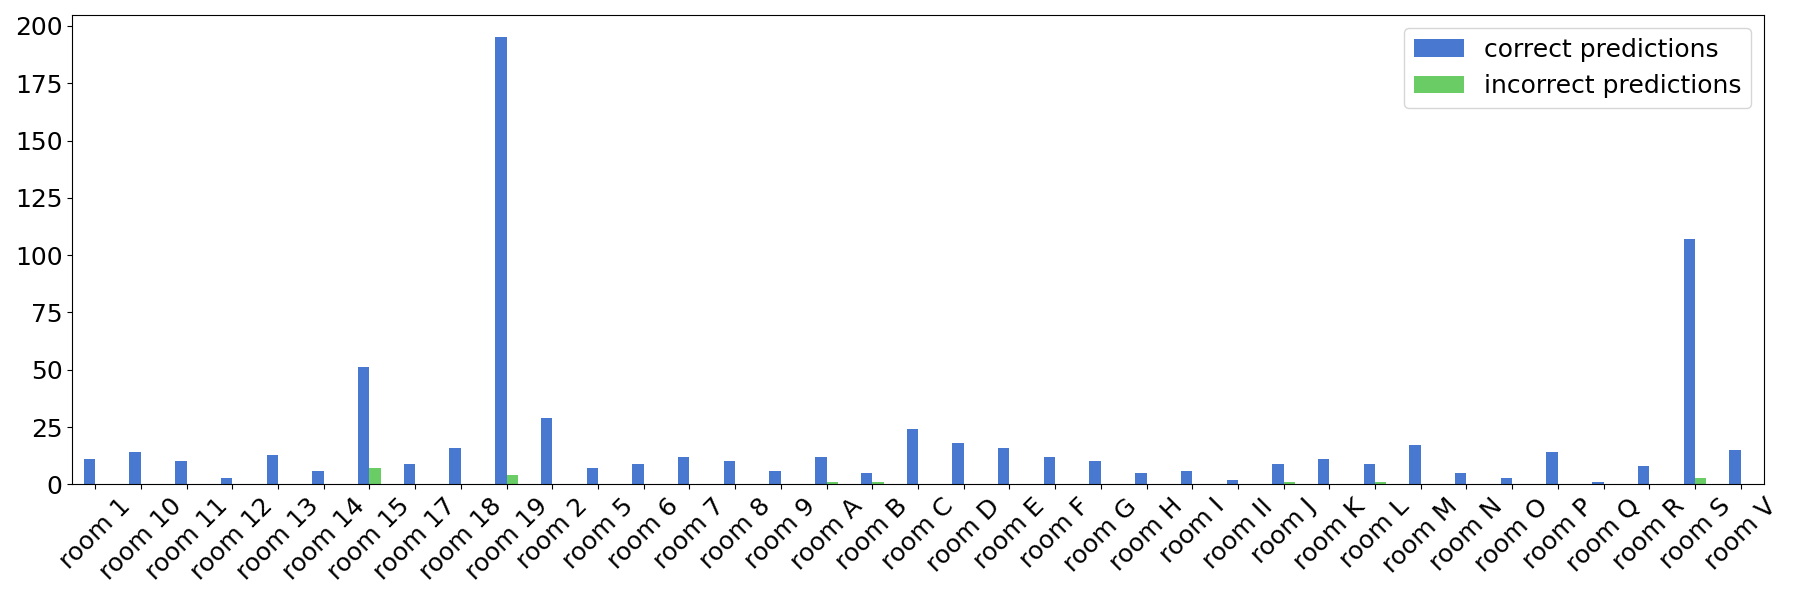
\includegraphics[width=\linewidth]{correct_and_incorrect.png}

    \caption{Correct and incorrect painting predictions per room}
    \label{fig:correct-incorrect-paintings}
\end{figure}

\section{Localization}
\label{sec:localization}

\subsection{Hidden Markov model}
\label{subsec:hidden-markov}

In order to establish an intelligent localization of the user by eliminating teleportations, a model inspired by the Hidden Markov model (\cite{eddy1996hidden}), was designed. The reason why no pure Hidden Markov can be used is because the input and output of the model is identical. Another reason is that there's no way to determine the initial room of any given video without having a number of observations, which are rooms in this case. Therefor an alternative Hidden Markov model was designed. \cite{jurafsky2014speech}

\subsection{Alternative Hidden Markov model}
\label{subsec:alternative-hidden-markov}

The alternative model basicly keeps a history of $n$ observations and predicts the most common observation as the current room. Initially the model doesn't know the current room and therefor doesn't emit any prediction until enough observations are obtained.

The model takes a list of probabilities per painting as an input which could possibly contain different probabilities for the same room. However the model needs one probability per room. So \formularef{eq:combine-chances} (\cite{genest1986combining}) is used to combine all probabilities for a given room into one probability. In this formula, $P(X = R)$ stands for the chance that the user is in room $R$, $P_{i}(X = R)$ stands for the $i^{th}$ chance, given by the prediction algorithm, that the user is in room $R$ and $P_{i}(X \ne R)$ is logically the chance that the user is not in room $R$.

\begin{equation}
    \label{eq:combine-chances}
    P(X = R) = \frac{\prod_{i} P_{test_i}(X = R)}{\prod_{i} P_{test_i}(X = R) + \prod_{i} P_{test_i}(X \ne R)}
\end{equation}

Although this formula can combine probabilities, it doesn't take the current room into account. Therefor a weight is added to each of the chances. This weight is equal to 1 when the room is accessible from within the current room and can be choosen for rooms that aren't accessible, the default is 0.5. This results in \formularef{eq:combine-chances-next-level}. If chances per room, e.g. from previous observations, are already known, then these are also taken into account in this calculation.

\begin{equation}
    \label{eq:combine-chances-next-level}
    P(X = R) = \frac{\prod_{i} w * P_{test_i}(X = R)}{\prod_{i} w * P_{test_i}(X = R) + \prod_{i} w * P_{test_i}(X \ne R)}
\end{equation}

By calculating the result of this formula per room, a list of probabilities per room is obtained. This list is then used to find the room with the highest probability which will be the observation for this input.

If the current observation is accessible from the current room, it is added to the history of observations. If this is not the case, the current room is added the history. Now, the most common room in the history is taken as the prediction for this input.

\section{Visualization}

In order to create a visualization of the algorithms described in the previous sections, a 3D model of the floor plan of the museum was created. First, this floor plan is converted into an SVG image so it can easily be altered in Python. Working this way makes it possible to dynamically create an HTML page showing the SVG floor plan and the currently analyzed frame along with the detected paintings. Because some operations need a lot of processing power, two separate processes are spawned. One process handles the painting detection, the other one handles the room prediction and the visualization of the HTML page in a webview. One of the major points of attention during the creation of the visualization was performance, hence the HTML file is never written to disk in order to bypass the I/O operations. Therefor the HTML page is always kept in memory. The detection process uses interprocess communication to send the detected paintings and the currently processed frame to the second process. This process then updates the Hidden Markov model as well as the HTML page and shows the result in a webview. An example of this webview is shown in \figureref{fig:webview}. Besides showing the floor plan and the image, other information is shown as well. This includes information about the predicted room, which is also visualized in red on the floor plan, a probability for this prediction, the currently processed video's name and the currently analyzed frame.

\begin{figure}
    \centering
    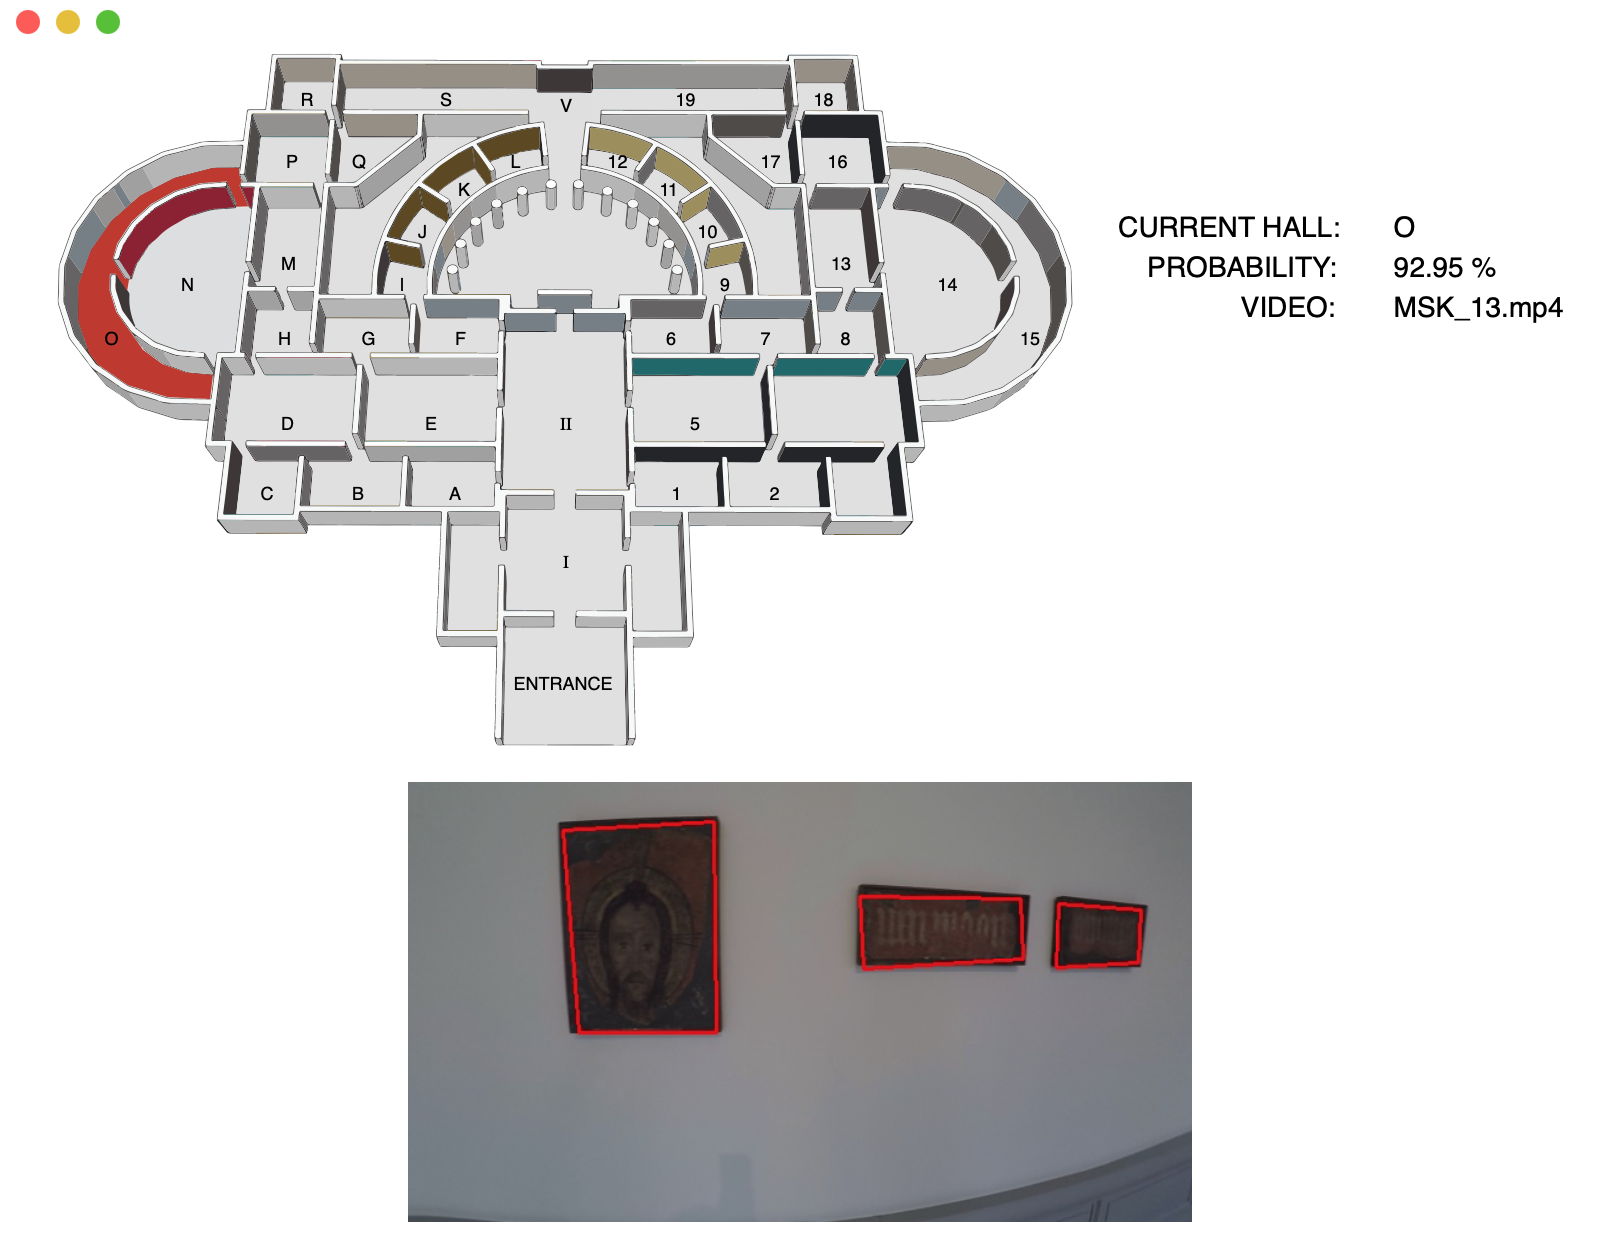
\includegraphics[width=0.7\linewidth]{visualization.png}
    \label{fig:webview}
    \caption{Modern visualization of the floor plan}
\end{figure}


%
% ---- Bibliography ----
%
% BibTeX users should specify bibliography style 'splncs04'.
% References will then be sorted and formatted in the correct style.
%
% TODO: is the style really necessary?
\bibliographystyle{splncs04}
\bibliography{references}

\end{document}
